\section{Fazit}

\subsection{�bersicht}

\begin{figure} [htbp]
	\centering
		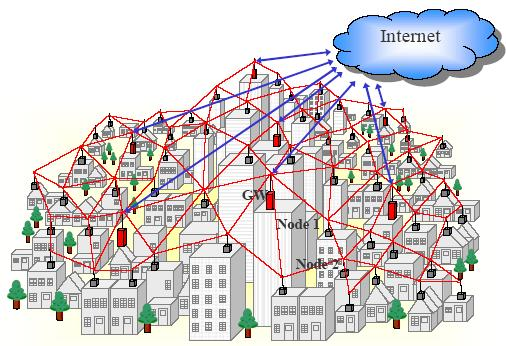
\includegraphics[width=0.50\textwidth]{WMN}
	\caption{Mesh Netz}
	\label{fig:WMN}
\end{figure}

\begin{verbatim}
  Position := Wurzel;  
  for i in 1..m do
    if (Position = Kante) then	
      if Zeichen auf dem Pfad im Baum = s'(i) then   
\end{verbatim}

Fachstudie
Hardwareplattformen und Systemsoftware f?r drahtlose vermaschte
Kommunikationsnetze

Bearbeiter:	Alex Egorenkov, Sergey Telejnikov, Valeri Schneider
Betreuer: Dipl.-Inf. Frank D?rr
Pr?fer: Prof. Dr. Kurt Rothermel
Zeitraum: November 2007 - Januar 2008

Hintergrund:
Ein drahtloses vermaschtes Netz (engl. Wireless Mesh Network, WMN) besteht aus einer Menge von Knoten, die ?ber drahtlose Kommunikationstechniken wie beispielsweise IEEE 802.11 Nachrichten austauschen. Die Vemaschung der Knoten erm?glicht dabei nicht nur den Austausch von Nachrichten zwischen unmittelbar benachbarten Knoten, sondern auch die Vermittlung von Nachrichten an entfernte Knoten ?ber mehrere Knoten hinweg. Die Vermittlungsfunktionalit?t wird dabei oft von dedizierten Vermittlungsknoten (engl. Mesh Router) bereitgestellt, die somit eine drahtlose Kommunikationsinfrastruktur f?r die Klienten (engt. Mesh Client) bilden. Durch den Einsatz vergleichsweise kosteng?nstiger Hardwarekomponenten und die Vermaschung der Knoten erm?glichen WMNs die kosteng?nstige Vernetzung auch gr??erer Gebiete. Entsprechende Netze, werden beispielsweise von Community-Projekten wie dein Freifunkprojekt oder Firmen wie Google bereits heute in der Praxis f?r den Aufbau gr??erer Netze eingesetzt, um beispielsweise kosteng?nstige Internetzug?nge f?r Stadtteile oder ganze St?dte zu realisieren.

WMNs sind auch f?r den Sonderforschungsbereichs (SFB) Nexus an der Universit?t Stuttgart von gro?em Interesse. Im Zentrum der Forschungen des SFB stehen Umgebungsmodelle f?r mobile kontextbezogene Systeme. Umgebungsmodelle sind digitale Abbilder der physischen Welt, die von kontextbezogenen Systemen genutzt werden, um sich selbst?ndig an die physische Umgebung des Benutzers anzupassen. Ein einfaches Beispiel sind ortsbezogene Anwendungen, die beispielsweise aufgrund der aktuellen geographischen Position eines Ger?ts automatisch Informationen ?ber nahe Restaurants. Sehensw?rdigkeiten, usw. selektieren k?nnen. Zur Kommunikation. insbesondere mit mobilen Ger?ten, werden dabei hybride Systeme betrachtet, in denen sowohl eine infrastrukturbasierte Kommunikation als auch die direkte Ad-hoc-Kommunikation zwischen mobilen Endsystemen m?glich ist. Hierbei spielen WMNs als eine spezielle Auspr?gung eines hybriden Kommunikationssystems eine wesentliche Rolle.
Aufgabenstellung:
F?r Forschungszwecke soll innerhalb des SFB Nexus ein WMN installiert werden. Dieses WMN dient einerseits Nexus-Anwendungen, insbesondere Anwendungen auf mobilen Ger?ten, als Kommunikationsmedium. Andererseits soll dieses WNIN auch als Testbed zur Erforschung verschiedene Erweiterungen von WMNs dienen, beispielsweise der Untersuchung neuartige kontextbezogener Kommunikationsmechanismen, der Erforschung von Publish/Subscribe-Diensten f?r WMNs oder der Verwaltung von Umgebungsmodellen innerhalb eines hybriden Systems wie es ein WMN darstellt. Ziel dieser Fachstudie ist die Ausarbeitung einer Empfehlung f?r die Beschaffung entsprechender Ger?te (Hardwareplattformen und Systemsoftware) f?r den Aufbau eines WMN.
Das Vorgehen umfasst im einzelnen:

"	 Einarbeitung in grundlegende WMN-Technologien.
"	 Analyse der Anforderungen des Nexus-Projektes an ein WNN.
"	 Erstellung einer ?bersicht ?ber aktuelle verf?gbare Hardwareplattformen und Systemsoftware f?r     WMN.
"	 Bewertung der analysierten Systeme hinsichtlich der ermittelten Anforderungen und Ausarbeitung einer Empfehlung f?r eine geeignetes WNN hinsichtlich Hardwareplattform und Systemsoftware.
Die Ergebnisse der Studie sind in einer schriftlichen Ausarbeitung zu dokumentieren und in einem Vortrag innerhalb des Abteilungskolloquiums vorzustellen.
2
'PV.5

